%-------------------------------------------------------------------------------
%	CAPITOLO 22
%-------------------------------------------------------------------------------

\chapter{La parola - Virtù del vino}
\subsection{La parola}
Si trattava di un buon diavolo, del tipo più vecchio che nuovo, per i suoi tempi. G. \: \:\footnote{Il nome è stato omesso} sensale da vino\footnote{Mediatore in contrattazioni di prodotti enologici}, reduce delle patrie battaglie\footnote{Reduce dalle guerre d'indipendenza italiana} era abbastanza introdotto\footnote{Disponeva di conoscenze o relazioni utili allo svolgimento della propria attività}, quantunque non fosse troppo magniloquente\footnote{Sebbene non fosse un gran oratore}.\\
\indent Un giorno nella cantina \index[Personaggi]{Mingazzi Fedele}Mingazzi, certo \index[Personaggi]{Allegri}Allegri di \index[Luoghi]{Glorie}Glorie doveva comprare una partita di vino. Il venditore chiedeva novanta lire, l'acquirente storceva il collo e premetteva meno, il sensale, con voce da basso profondo chiede: "La parola a me", prende le mani del venditore e dell'acquirente e con le sue le stringe fortemente imprimendo il colpo, finale solito, per la conclusione e sillaba: <<Zdot scud\footnote{<<Diciotto scudi>>. Equivalevano a 90 Lire.}>>.\\
\indent Una risata accolse tale sproposito, ma il contratto si fece su altre basi.
\newpage
\subsection{Virtù del vino}
È sempre il nostro uomo che parla.\\
\indent Un giorno parlando con una maestra chiese: <<L'an ha mai avù fiùl?\footnote{<<Non ha mai avuto figli?>>}>>\\
\indent La maestra: <<No>>.\\
\indent Il nostro G: <<Alora cla beva de ven négar gros sl'in vó mètar in sê\footnote{<<Allora beva del vino nero grosso se vuole farne>>}>>.\\
\indent Farmacisti e medici aprite questa ricetta alla terapia. 

\begin{figure}[htb]
    \centering
    %\vspace{-0.7cm}
    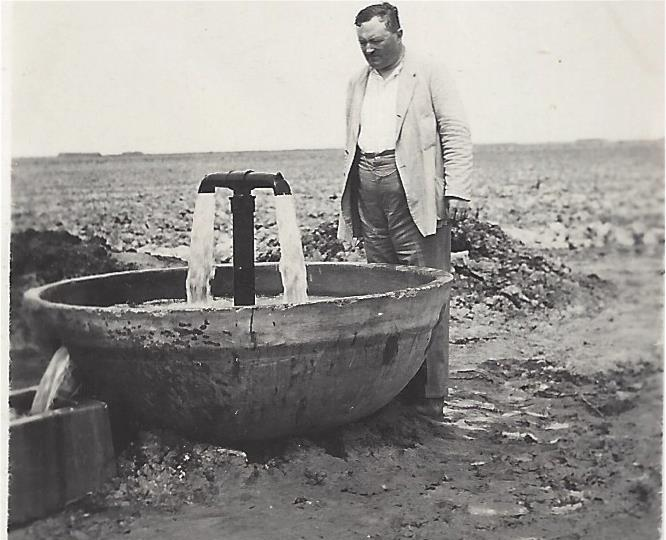
\includegraphics[width=\textwidth]{ambaradam}
    \caption[Mingazzi durante lavoro di bonifica]{Mingazzi\index[Personaggi]{Mingazzi Stefano} durante un lavoro di bonifica in una delle sue proprietà, Amba Aradam\label{fig:ambaradam}. La vasca presente nella foto si trova attualmente nel giardino di Mariannina Gagliardi\index[Personaggi]{Gagliardi Mariannina (n. 1927)}.}
    %\vspace{-0.3cm}
\end{figure}